\section{Limpieza de HUD y ruido}
\label{sec:limpieza}
% Responsable: Laura Martínez-Galindo

Esta etapa entrega tres versiones del mismo conjunto de imágenes anotadas: \texttt{dataset\_original} (el frame exacto del video), \texttt{dataset\_sin\_hud} y \texttt{dataset\_denoised}. Como no existe una versión limpia de los videos, todo el proceso es autosupervisado y se evalúa con métricas sin referencia y revisión visual. Los resultados se reportan por imagen, como distribuciones, y no como promedios.

\subsection{Entendimiento de los datos}

\subsubsection{Correspondencia entre las imágenes anotadas y los videos}
Las imágenes anotadas provenían de tres conjuntos previos, en JPEG, reescaladas, algunas con realce y sin número de frame. Para limpiarlas con información temporal y a la calidad original fue necesario ubicar el frame exacto del que salió cada una:

\begin{enumerate}
    \item \textbf{Búsqueda gruesa.} Cada imagen se compara, reducida y sin la zona del HUD, contra un índice de miniaturas de los tres videos.
    \item \textbf{Búsqueda fina.} Se refina en una ventana de frames alrededor del mejor candidato.
    \item \textbf{Verificación.} Cuando la imagen es casi idéntica al frame se verifica píxel a píxel (PSNR); cuando fue recomprimida o realzada se verifica con la textura de alta frecuencia, que no cambia con el contraste.
\end{enumerate}

Las 1.116 imágenes quedaron emparejadas con su frame (359 verificadas píxel a píxel, 756 por textura y 1 ambigua por tratarse de una escena casi quieta). Se excluyeron 712 imágenes que pertenecen a otro vuelo, no incluido en los tres videos, y se fusionaron 22 repetidas. El conjunto final tiene 6.088 cajas en cinco clases (\fref{tab:clases}) y está dominado por el video 2, que aporta 839 imágenes y el 87\,\% de las cajas. La \fref{fig:dataset_donde} muestra de qué parte de cada video salen las imágenes.

\begin{table}[H]
\centering
\small
\caption{Cajas anotadas por clase y video en el conjunto final (1.116 imágenes).}
\label{tab:clases}
\begin{tabular}{lrrrr}
\toprule
\textbf{Clase} & \textbf{Video 1} & \textbf{Video 2} & \textbf{Video 3} & \textbf{Total} \\
\midrule
Edificación & 249 & 3.347 & 101 & 3.697 \\
Vía & 9 & 1.392 & 30 & 1.431 \\
Vehículo & 0 & 520 & 9 & 529 \\
SDZI & 92 & 0 & 149 & 241 \\
Río & 78 & 35 & 77 & 190 \\
\midrule
Total & 428 & 5.294 & 366 & 6.088 \\
\bottomrule
\end{tabular}
\end{table}

\begin{figure}[H]
\centering
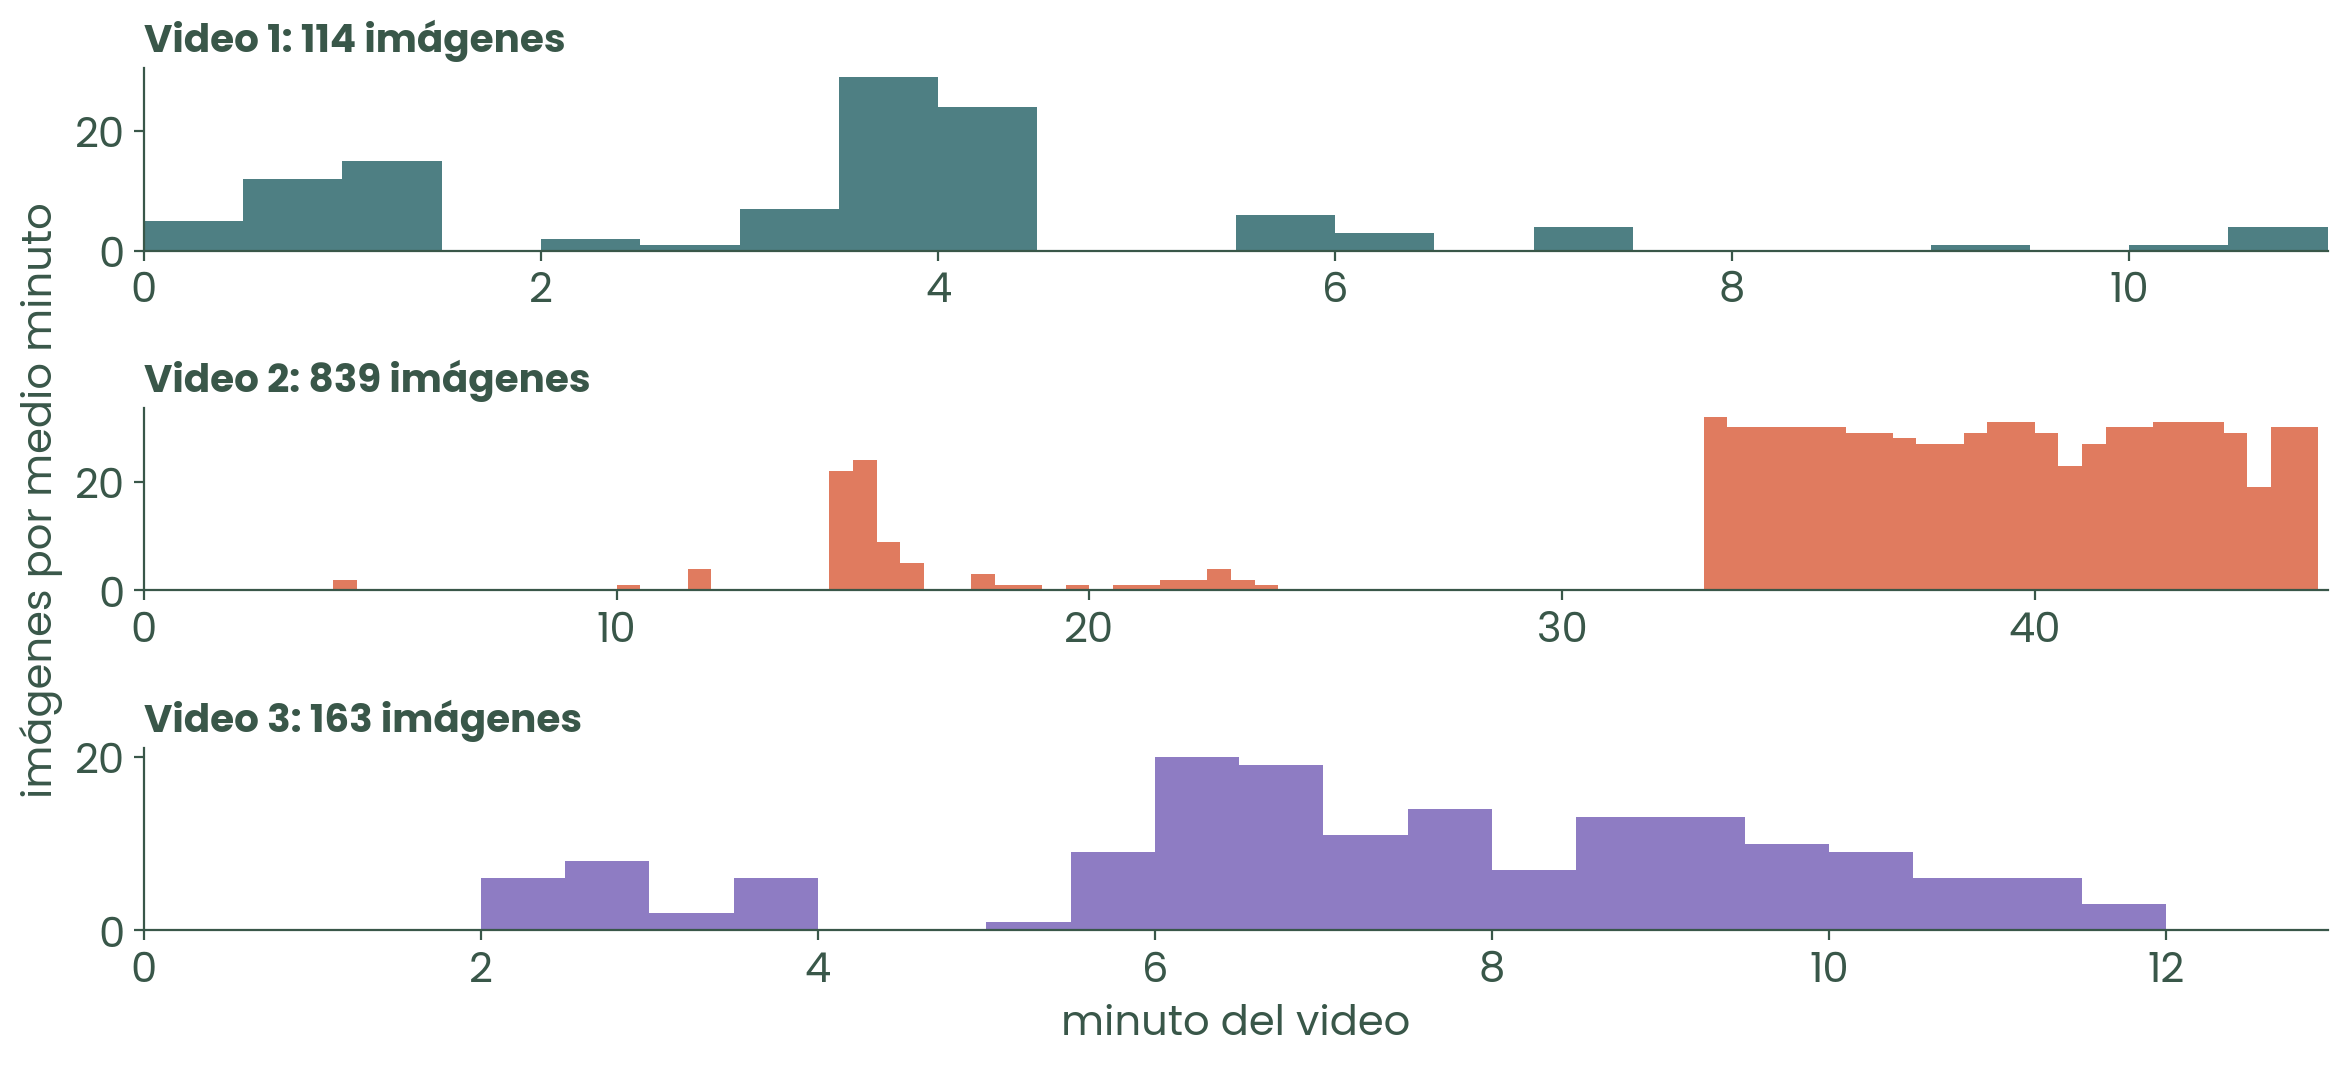
\includegraphics[width=0.85\textwidth]{figures/limpieza/dataset_de_donde.png}
\caption{Minuto de cada video del que sale cada imagen del conjunto final.}
\label{fig:dataset_donde}
\end{figure}

\subsubsection{Régimen de operación del sensor}
La cámara combina varios sensores y filtros de realce, y la combinación activa (el \textit{régimen}) aparece escrita en una esquina del HUD. En lugar de inferirla con heurísticas de color, se lee directamente: cada línea de esa esquina se compara con plantillas del texto, en uno de cada 15 frames. Si una línea no se parece a ninguna plantilla se marca como desconocida, se guarda su recorte, se agrega la plantilla y se vuelve a leer. Una lectura solo vale si coincide con la anterior y la siguiente, de modo que las transiciones no se usan.

Se encontraron ocho regímenes y ningún frame quedó sin leer. En cada video predomina uno, y los tres corresponden al sensor visible con distintos filtros; en este documento se identifican como A, B y C (\fref{fig:regimenes}). El régimen B ocupa el 91\,\% del video 1, el A el 84\,\% del video 2 y el C el 90\,\% del video 3. Entre los tres cubren 1.082 de las 1.116 imágenes (97\,\%): 823 del régimen A, 162 del C y 97 del B. Las 34 restantes pertenecen a regímenes minoritarios (térmico, baja luz e infrarrojo de onda corta).

\begin{figure}[H]
\centering
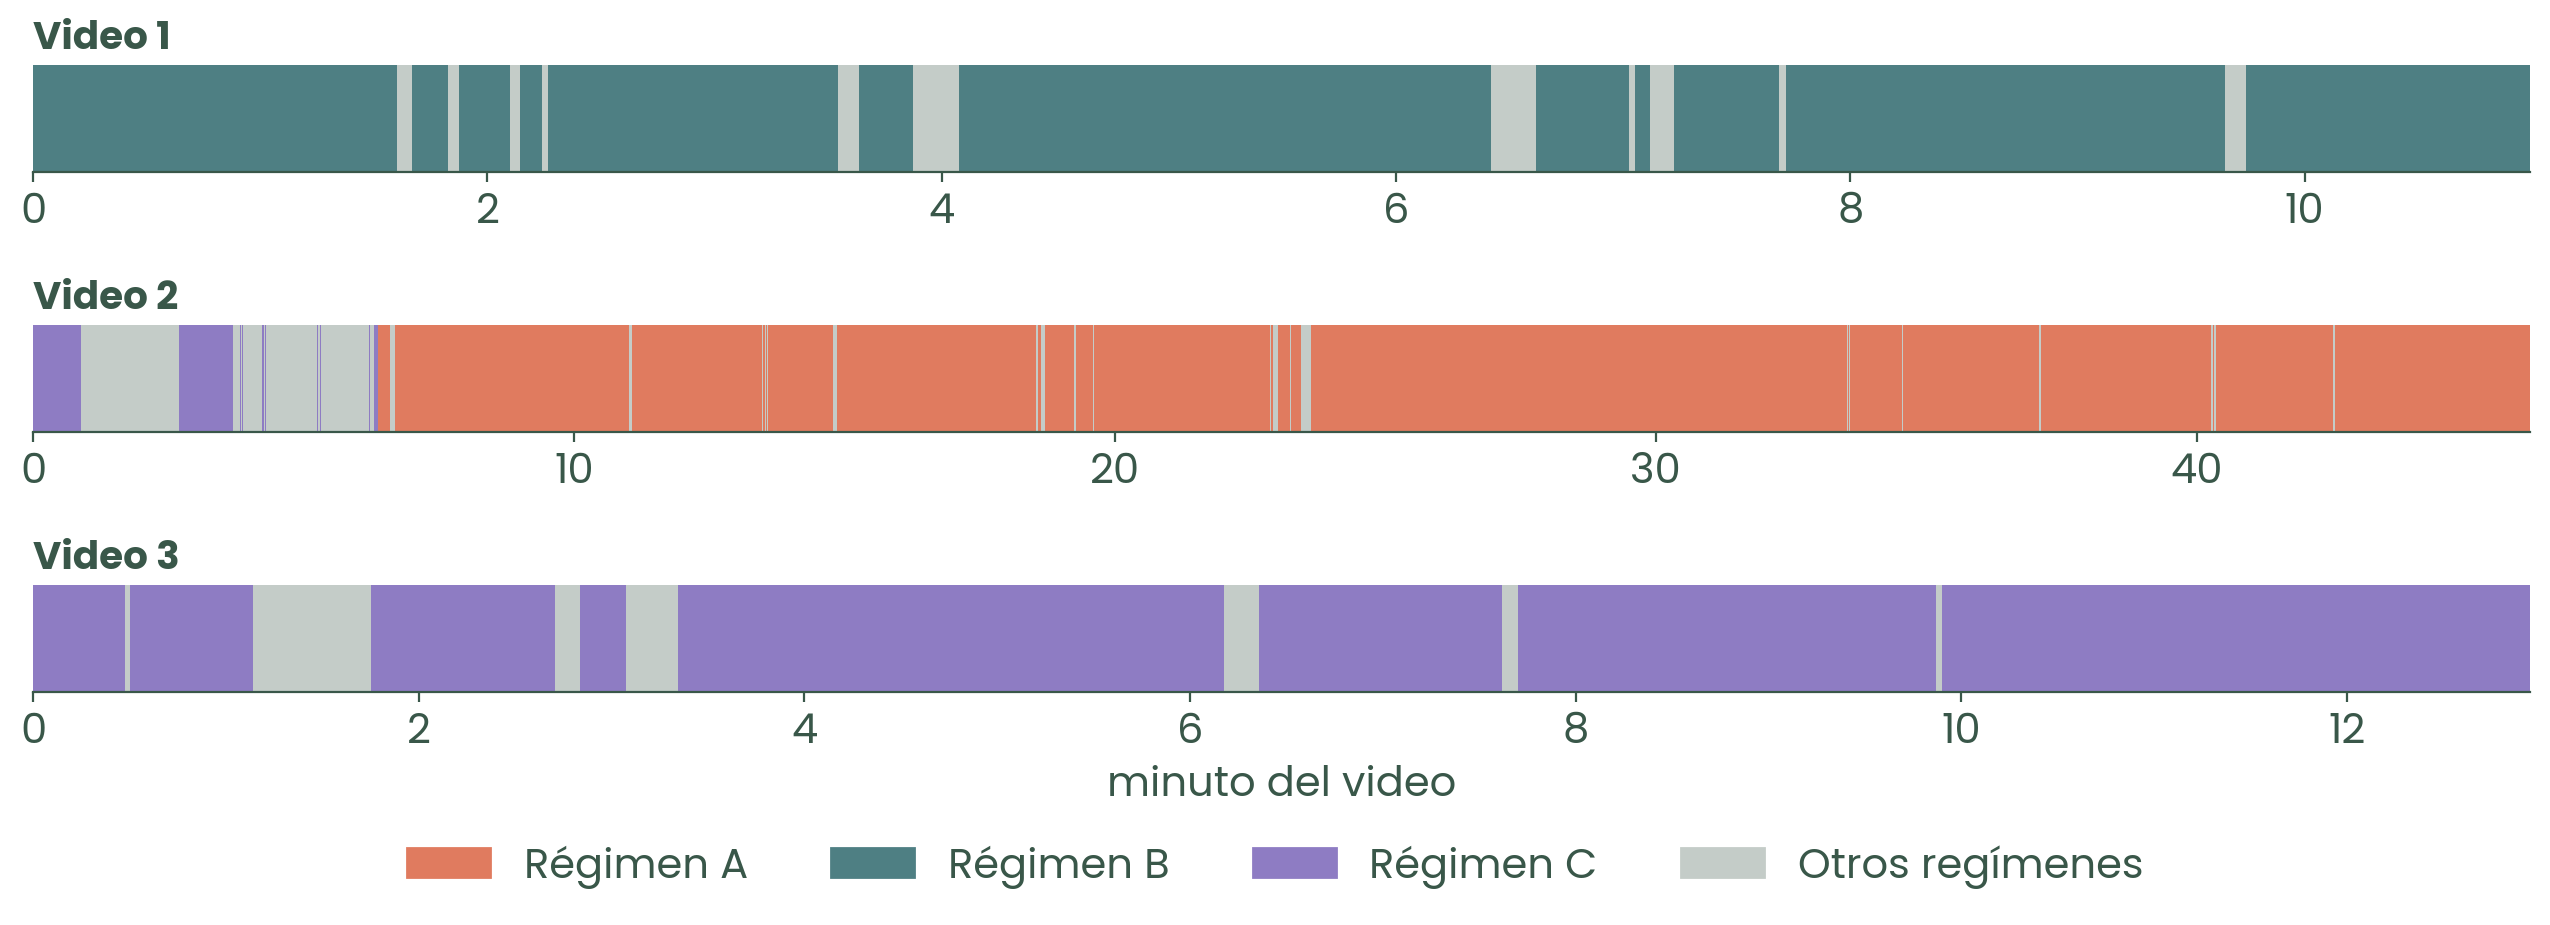
\includegraphics[width=0.9\textwidth]{figures/limpieza/regimenes_tiempo.png}\\[0.3cm]
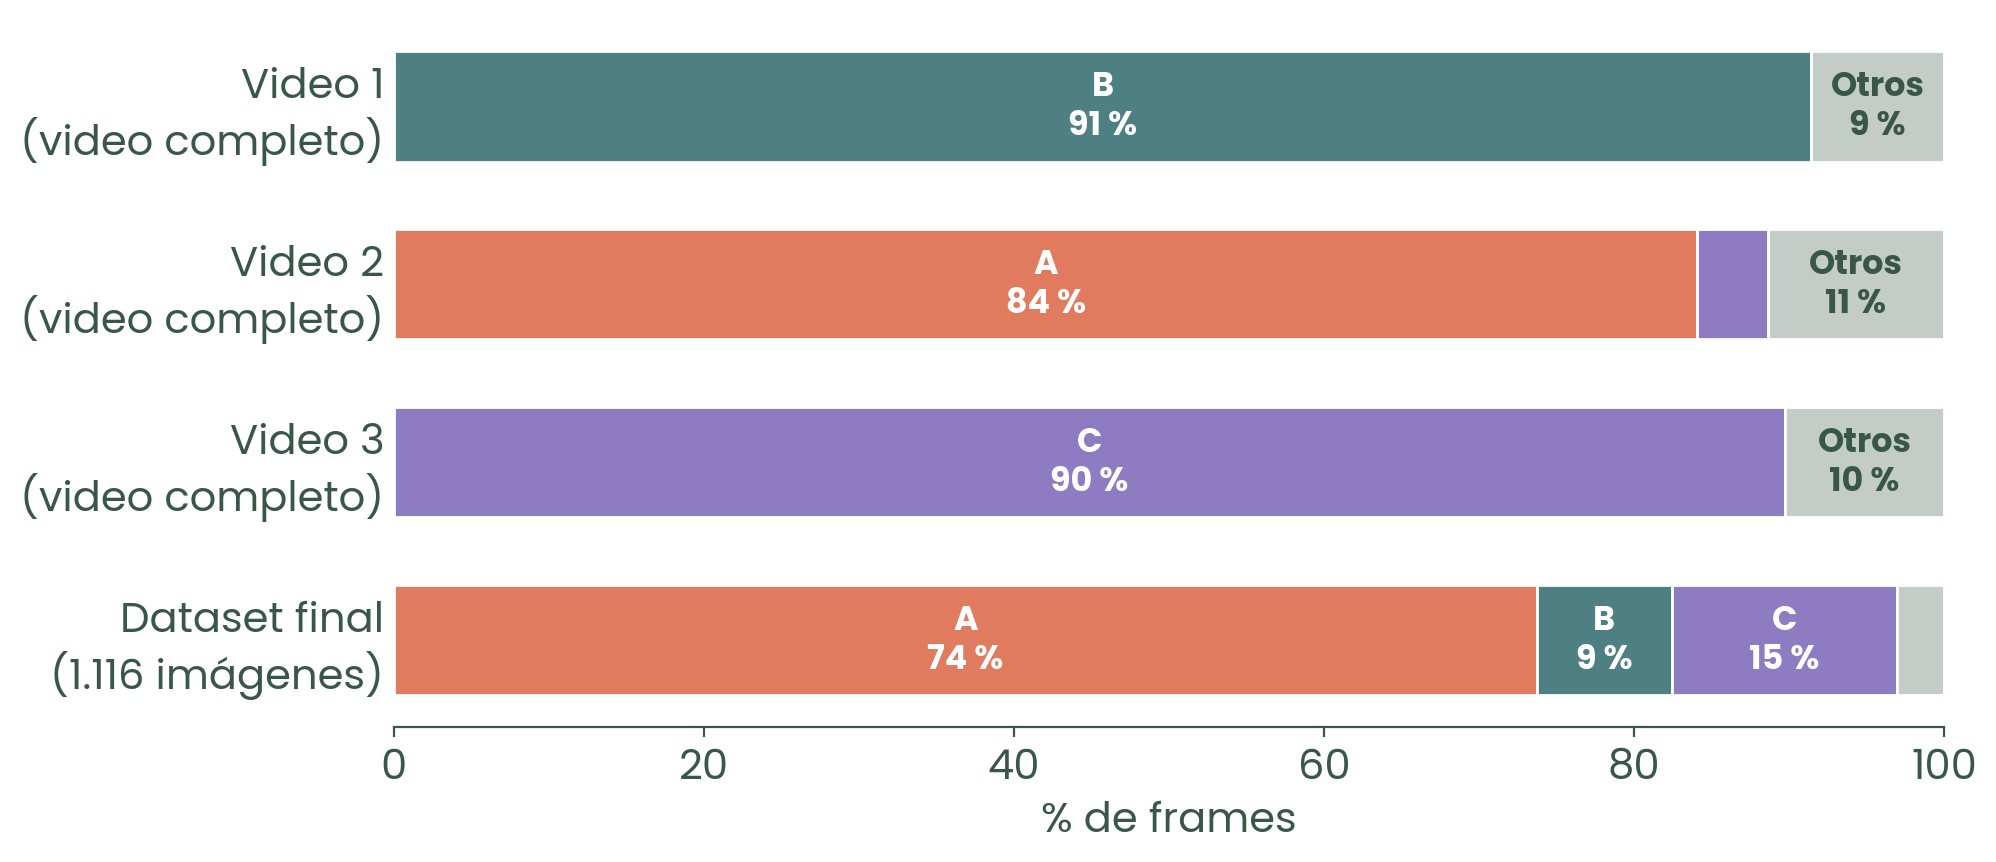
\includegraphics[width=0.75\textwidth]{figures/limpieza/regimenes_pct.png}
\caption{Régimen del sensor a lo largo de cada video (arriba) y porcentaje de cada régimen en los videos completos y en el conjunto final (abajo).}
\label{fig:regimenes}
\end{figure}

\subsubsection{Caracterización del ruido por régimen}
Para cada régimen se tomaron 60 frames repartidos en todos sus tramos y, fuera del HUD y de los bordes de la escena, se midió: el nivel de ruido $\sigma$ con el estimador de Immerkær~\cite{immerkaer1996fast}, la correlación del ruido con el píxel vecino a 1 y 2 píxeles (horizontal y vertical), el porcentaje de píxeles tipo sal y pimienta y la intensidad de los bloques de compresión. La \fref{tab:ruido} y la \fref{fig:ruido_regimen} resumen los tres regímenes dominantes.

\begin{table}[H]
\centering
\small
\caption{Ruido de los regímenes dominantes: mediana por régimen sobre 60 frames (para $\sigma$ también el rango p25--p75).}
\label{tab:ruido}
\begin{tabular}{lcccccc}
\toprule
\textbf{Régimen} & \textbf{$\sigma$ p50 [p25--p75]} & \textbf{Corr. horiz.} & \textbf{Corr. vert.} & \textbf{Corr. 2 px} & \textbf{Sal y pim.} & \textbf{Bloques} \\
\midrule
A (video 2) & 4,89 [3,58--6,71] & 0,35 & 0,32 & $-$0,03 & 3,57\,\% & 1,36 \\
B (video 1) & 0,36 [0,28--0,44] & 0,50 & 0,43 & 0,25 & 0,00\,\% & 1,23 \\
C (video 3) & 0,24 [0,15--0,36] & 0,43 & 0,43 & 0,21 & 0,00\,\% & 1,91 \\
\bottomrule
\end{tabular}
\end{table}

\begin{figure}[H]
\centering
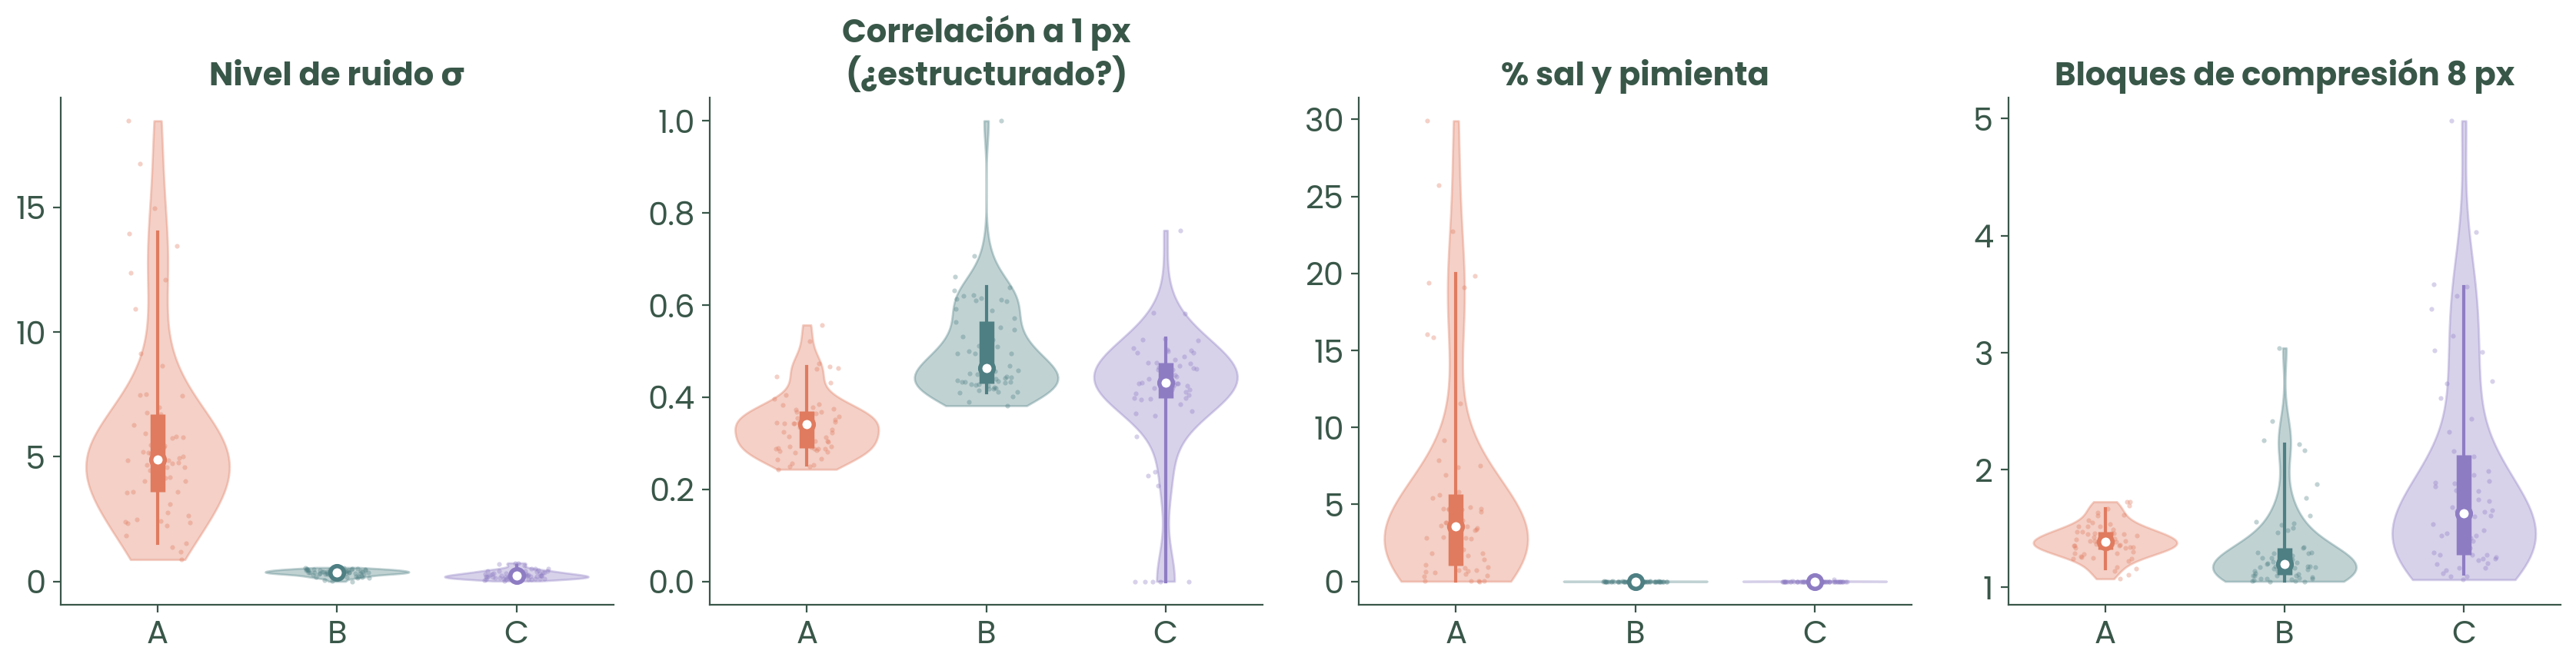
\includegraphics[width=\textwidth]{figures/limpieza/ruido_regimen_dist.png}
\caption{Distribución de las características del ruido en los tres regímenes dominantes. Cada punto es un frame.}
\label{fig:ruido_regimen}
\end{figure}

\begin{figure}[H]
\centering
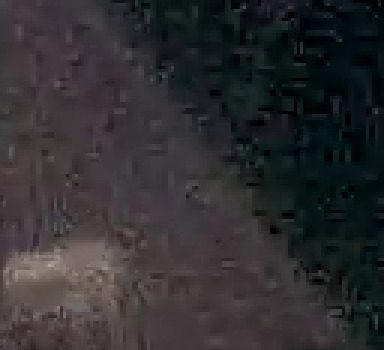
\includegraphics[height=3.4cm]{figures/limpieza/ruido_regimen_A.jpg}\hfill
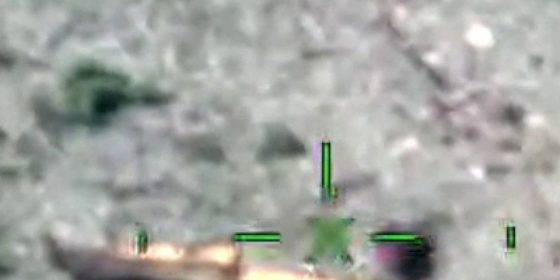
\includegraphics[height=3.4cm]{figures/limpieza/ruido_regimen_B.jpg}\\[0.2cm]
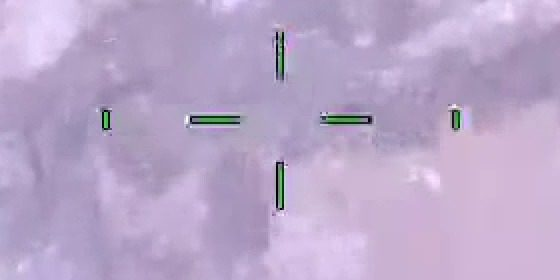
\includegraphics[height=3.4cm]{figures/limpieza/ruido_regimen_C.jpg}
\caption{Recortes ampliados del ruido en los regímenes A (arriba, izquierda), B (arriba, derecha) y C (abajo).}
\label{fig:ruido_recortes}
\end{figure}

De esta medición salen las decisiones de modelado:
\begin{itemize}
    \item \textbf{El tipo de ruido lo define el régimen.} En A el ruido es alto, de grano fino casi independiente entre píxeles y con impulsos; en B y C es bajo y correlacionado con el vecino (en grumos), y en C además dominan los bloques de compresión.
    \item \textbf{El nivel también depende del video.} Un mismo régimen medido en dos videos mostró 4,5 veces más ruido en el video 2, que es el más comprimido.
    \item \textbf{Un punto ciego de un solo píxel no alcanza} cuando el ruido se parece al del vecino: la red puede copiarlo. Por eso en B y C se requieren métodos que rompan esa correlación.
    \item \textbf{En B y C el ruido está cerca del límite de cuantización de 8 bits} ($\approx 0{,}3$ niveles de gris), es decir, casi no se ve.
\end{itemize}

\subsection{Eliminación del HUD}

\subsubsection{Máscara}
El HUD se segmenta con una heurística en tres pasos: (1) umbral de verde saturado en el espacio HSV; (2) un acumulador temporal de 250 frames que conserva solo los píxeles persistentes, porque el HUD permanece fijo en pantalla mientras el terreno se mueve, lo que descarta la vegetación verde; y (3) operaciones morfológicas con una dilatación de $3\times3$ para cubrir los bordes del texto.

\subsubsection{Inpainting}
La región enmascarada se reconstruye con ProPainter~\cite{zhou2023propainter}, que completa el flujo óptico dentro de la máscara, propaga píxeles reales desde los frames donde esa porción del terreno no estaba cubierta y rellena con un transformer espacio-temporal lo que nunca se vio. El resultado se guarda en modo compuesto: el frame final es el original y solo los píxeles de la máscara provienen de ProPainter. Así el ruido del resto de la imagen queda intacto para la etapa siguiente.

\subsubsection{Resultados}
La reducción se mide por imagen como el porcentaje de píxeles verdes del HUD que desaparecen. El HUD ocupa una fracción pequeña del frame: la mediana es de 0,35\,\% en el video 1, 1,08\,\% en el video 2 y 0,78\,\% en el video 3 (\fref{fig:hud}). La \fref{tab:hud} presenta la distribución de la reducción. La meta del 80\,\% se cumple en 1.115 de las 1.116 imágenes; el único caso por debajo es un frame del video 2 en el que el relleno dejó un borde verdoso. Lo que permanece en las demás son bordes y verde real del paisaje.

\begin{table}[H]
\centering
\small
\caption{Porcentaje de píxeles del HUD eliminados por imagen.}
\label{tab:hud}
\begin{tabular}{lrcccc}
\toprule
\textbf{Video} & \textbf{Imágenes} & \textbf{Mediana} & \textbf{p25--p75} & \textbf{p5} & \textbf{Mínimo} \\
\midrule
Video 1 & 114 & 98,4\,\% & 97,8--99,0\,\% & 95,7\,\% & 82,1\,\% \\
Video 2 & 839 & 98,6\,\% & 98,2--99,0\,\% & 95,9\,\% & 68,9\,\% \\
Video 3 & 163 & 98,6\,\% & 98,1--99,8\,\% & 97,5\,\% & 91,8\,\% \\
\bottomrule
\end{tabular}
\end{table}

\begin{figure}[H]
\centering
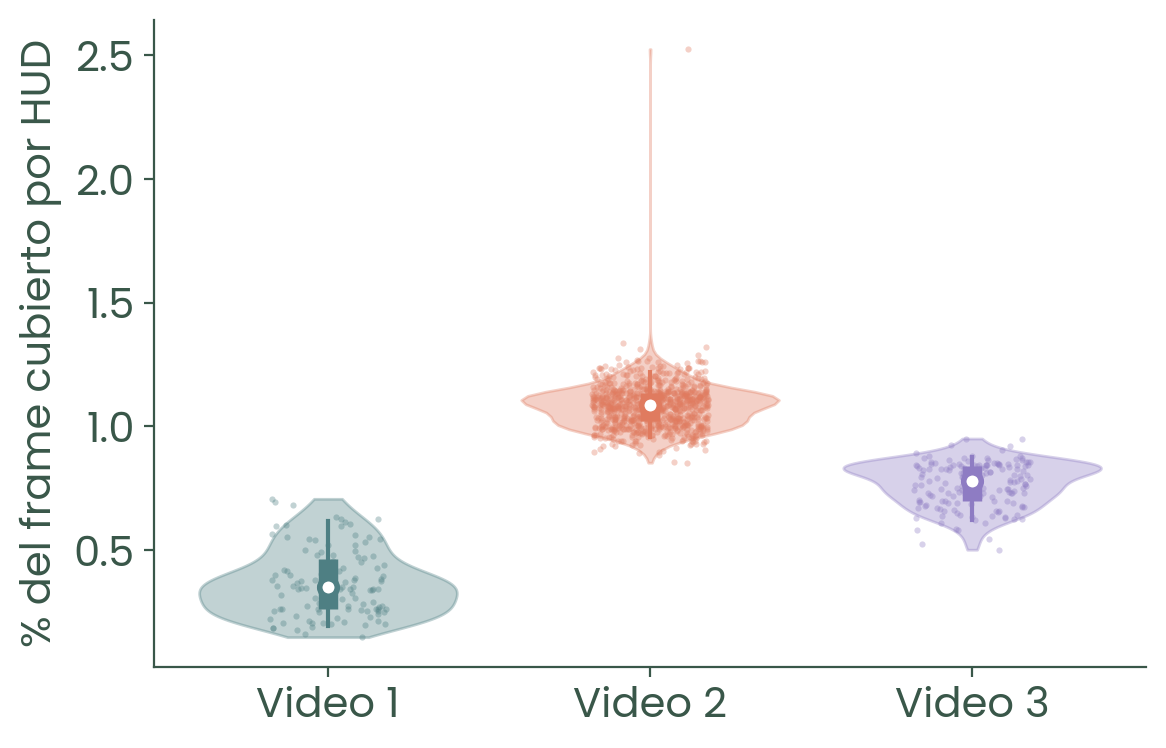
\includegraphics[width=0.48\textwidth]{figures/limpieza/hud_area_dist.png}\hfill
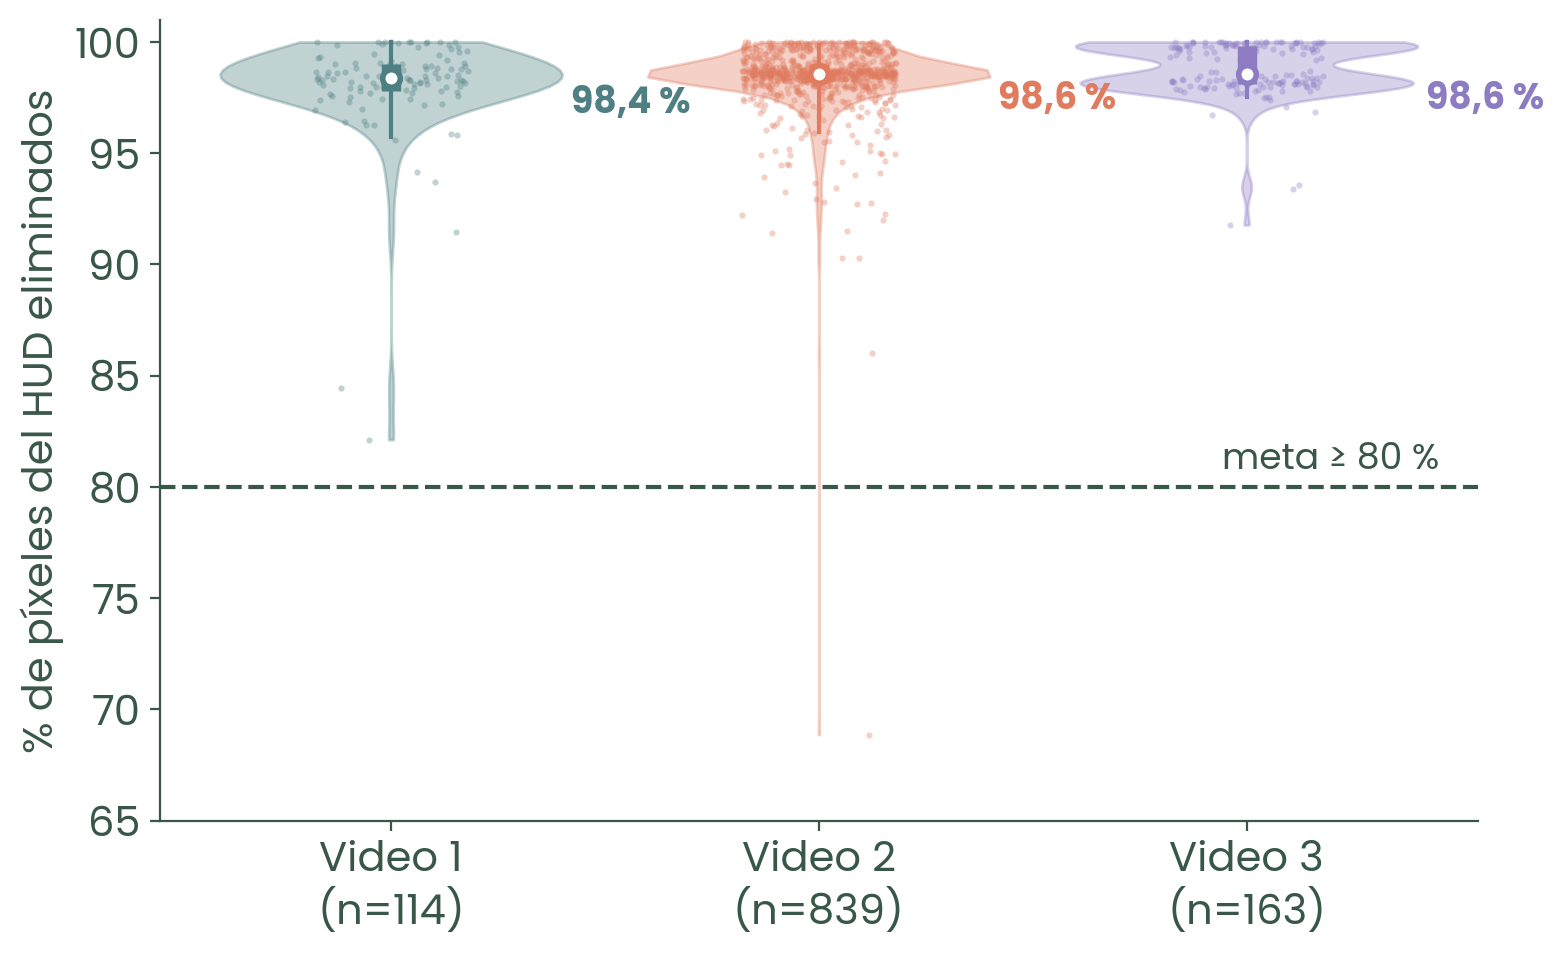
\includegraphics[width=0.48\textwidth]{figures/limpieza/hud_reduccion_dist.png}
\caption{Área del frame cubierta por el HUD (izquierda) y porcentaje de píxeles del HUD eliminados (derecha). Cada punto es una imagen del conjunto final.}
\label{fig:hud}
\end{figure}

La \fref{fig:hud_ejemplos} muestra dos ejemplos del resultado.

\begin{figure}[H]
\centering
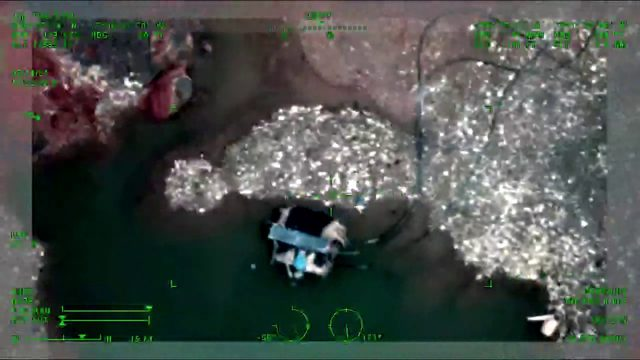
\includegraphics[width=0.32\textwidth]{figures/limpieza/ej_hud_original.jpg}\hfill
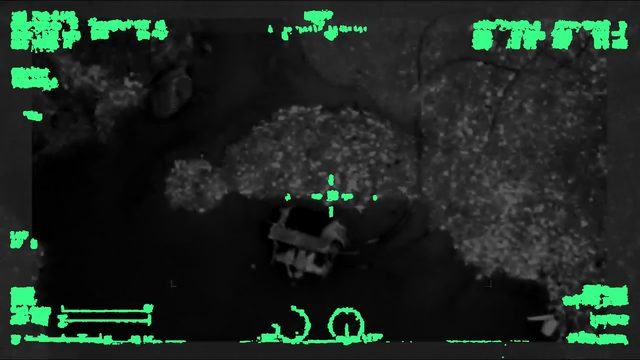
\includegraphics[width=0.32\textwidth]{figures/limpieza/ej_hud_mascara.jpg}\hfill
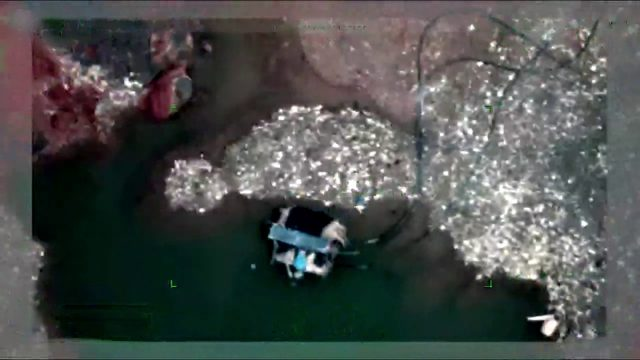
\includegraphics[width=0.32\textwidth]{figures/limpieza/ej_hud_sin.jpg}\\[0.2cm]
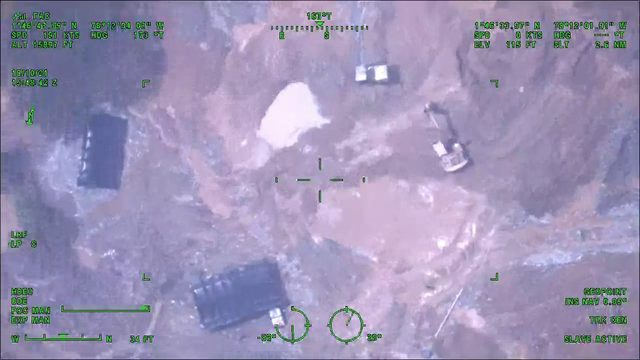
\includegraphics[width=0.32\textwidth]{figures/limpieza/ej_hud_v3_original.jpg}\hspace{0.02\textwidth}
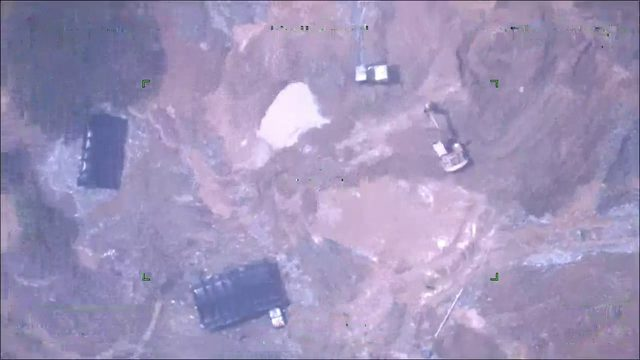
\includegraphics[width=0.32\textwidth]{figures/limpieza/ej_hud_v3_sin.jpg}
\caption{Eliminación del HUD. Arriba, un frame del video 1: original, píxeles que entran a la máscara y resultado. Abajo, un frame del video 3: original y resultado. Las imágenes se muestran a resolución reducida.}
\label{fig:hud_ejemplos}
\end{figure}

\subsection{Reducción de ruido}

\subsubsection{Fase exploratoria}
En una primera fase se probaron métodos espaciales (Noise2Noise~\cite{lehtinen2018noise2noise}, Noise2Void~\cite{krull2019noise2void}, StructN2V~\cite{broaddus2020structn2v}, Neighbor2Neighbor~\cite{huang2021neighbor2neighbor} y Blind2Unblind~\cite{wang2022blind2unblind}), temporales (UDVD~\cite{sheth2021udvd} y Frames2Residual~\cite{ji2026frames2residual}, entre otros) y ensambles, entrenados sobre fragmentos de video sin separar por régimen. Esta fase dejó dos hallazgos que cambiaron el diseño:

\begin{itemize}
    \item \textbf{El mejor modelo cambiaba de un video a otro}, lo que llevó a caracterizar el ruido por régimen.
    \item \textbf{NIQE y BRISQUE por sí solas premian el desenfoque.} Los modelos que más las bajaban en el video 2 conservaban apenas una fracción de la nitidez original. Por eso la selección combina esas métricas con medidas de conservación de detalle y de color, y con revisión visual.
\end{itemize}

\subsubsection{Diseño experimental por régimen}
Se busca el mejor modelo para cada régimen dominante por separado. Todos los métodos comparten el mismo protocolo:

\begin{itemize}
    \item \textbf{Entrenamiento.} 1.500 frames del régimen tomados de los videos completos, equiespaciados en todos sus tramos, con 4.000 pasos y los hiperparámetros del artículo de cada método. Los parches se sortean fuera del HUD.
    \item \textbf{Separación.} Se excluyen los 90 frames anteriores y posteriores (3 segundos) a cada imagen del conjunto anotado, de modo que en la fase de selección el modelo no ve las imágenes que va a limpiar.
    \item \textbf{Evaluación.} Hasta 300 imágenes del conjunto sin HUD por régimen, con los píxeles del HUD excluidos de las métricas.
\end{itemize}

La comparación se hizo en tres rondas. La primera cubrió UDVD, AP-BSN~\cite{lee2022apbsn}, MM-BSN~\cite{zhang2023mmbsn}, Neighbor2Neighbor, Blind2Unblind y la línea base clásica de medias no locales~\cite{buades2005nlm}. La segunda se concentró en el régimen A y agregó métricas de grano y de fidelidad de color. La tercera amplió la comparación a 47 métodos en los tres regímenes (141 experimentos): redes de punto ciego, métodos autosupervisados por pares o máscaras, transformers, métodos \textit{zero-shot} que entrenan una red por imagen, métodos temporales que usan los frames vecinos, filtros clásicos de referencia y ensambles de los tres mejores de cada régimen.

\subsubsection{Métricas}
\begin{itemize}
    \item \textbf{NIQE~\cite{mittal2013making} y BRISQUE~\cite{mittal2012noreference}}: calidad sin referencia; menor es mejor. Meta de la propuesta: reducción de al menos 8\,\% frente a la imagen sin procesar.
    \item \textbf{Grano y $\sigma$ residual}: ruido que queda después de limpiar.
    \item \textbf{Conservación de bordes y correlación del residuo con los bordes}: si lo que el modelo quitó tiene la forma de la escena, borró detalle.
    \item \textbf{Fidelidad de color}: razón de croma y diferencia de color frente a la entrada.
    \item \textbf{Métricas temporales}: \textit{warping error} (parpadeo entre frames alineados por flujo óptico) y una estimación insesgada del PSNR calculada contra frames vecinos ruidosos.
\end{itemize}
Un método se descarta si altera el color, y la pérdida de bordes se revisa visualmente en recortes a tamaño real.

\subsubsection{Resultados}
\paragraph{Primera ronda.} La \fref{fig:ronda1} muestra, por imagen, el ruido que queda y la fracción de bordes conservados con cada método (97 imágenes del régimen B y 120 de los regímenes A y C). En el régimen A la mediana de $\sigma$ pasa de 5,4 sin limpiar a 0,7 con UDVD, 0,9 con Blind2Unblind y 1,0 con AP-BSN, mientras Neighbor2Neighbor y el filtro clásico casi no la cambian (3,6 y 3,3). AP-BSN lo logra a costa del detalle: conserva una mediana de 0,49 de los bordes. En los regímenes B y C el ruido de partida ya está junto al límite visible (medianas de 0,43 y 0,35) y ningún método lo baja de forma apreciable sin perder bordes: UDVD conserva una mediana de 0,71 en B y de 0,34 en C. La medida de bordes de esta ronda cuenta el grano como borde, por lo que en el régimen A favorece a los métodos que limpian poco; esto motivó las métricas de grano y de color de la segunda ronda.

\begin{figure}[H]
\centering
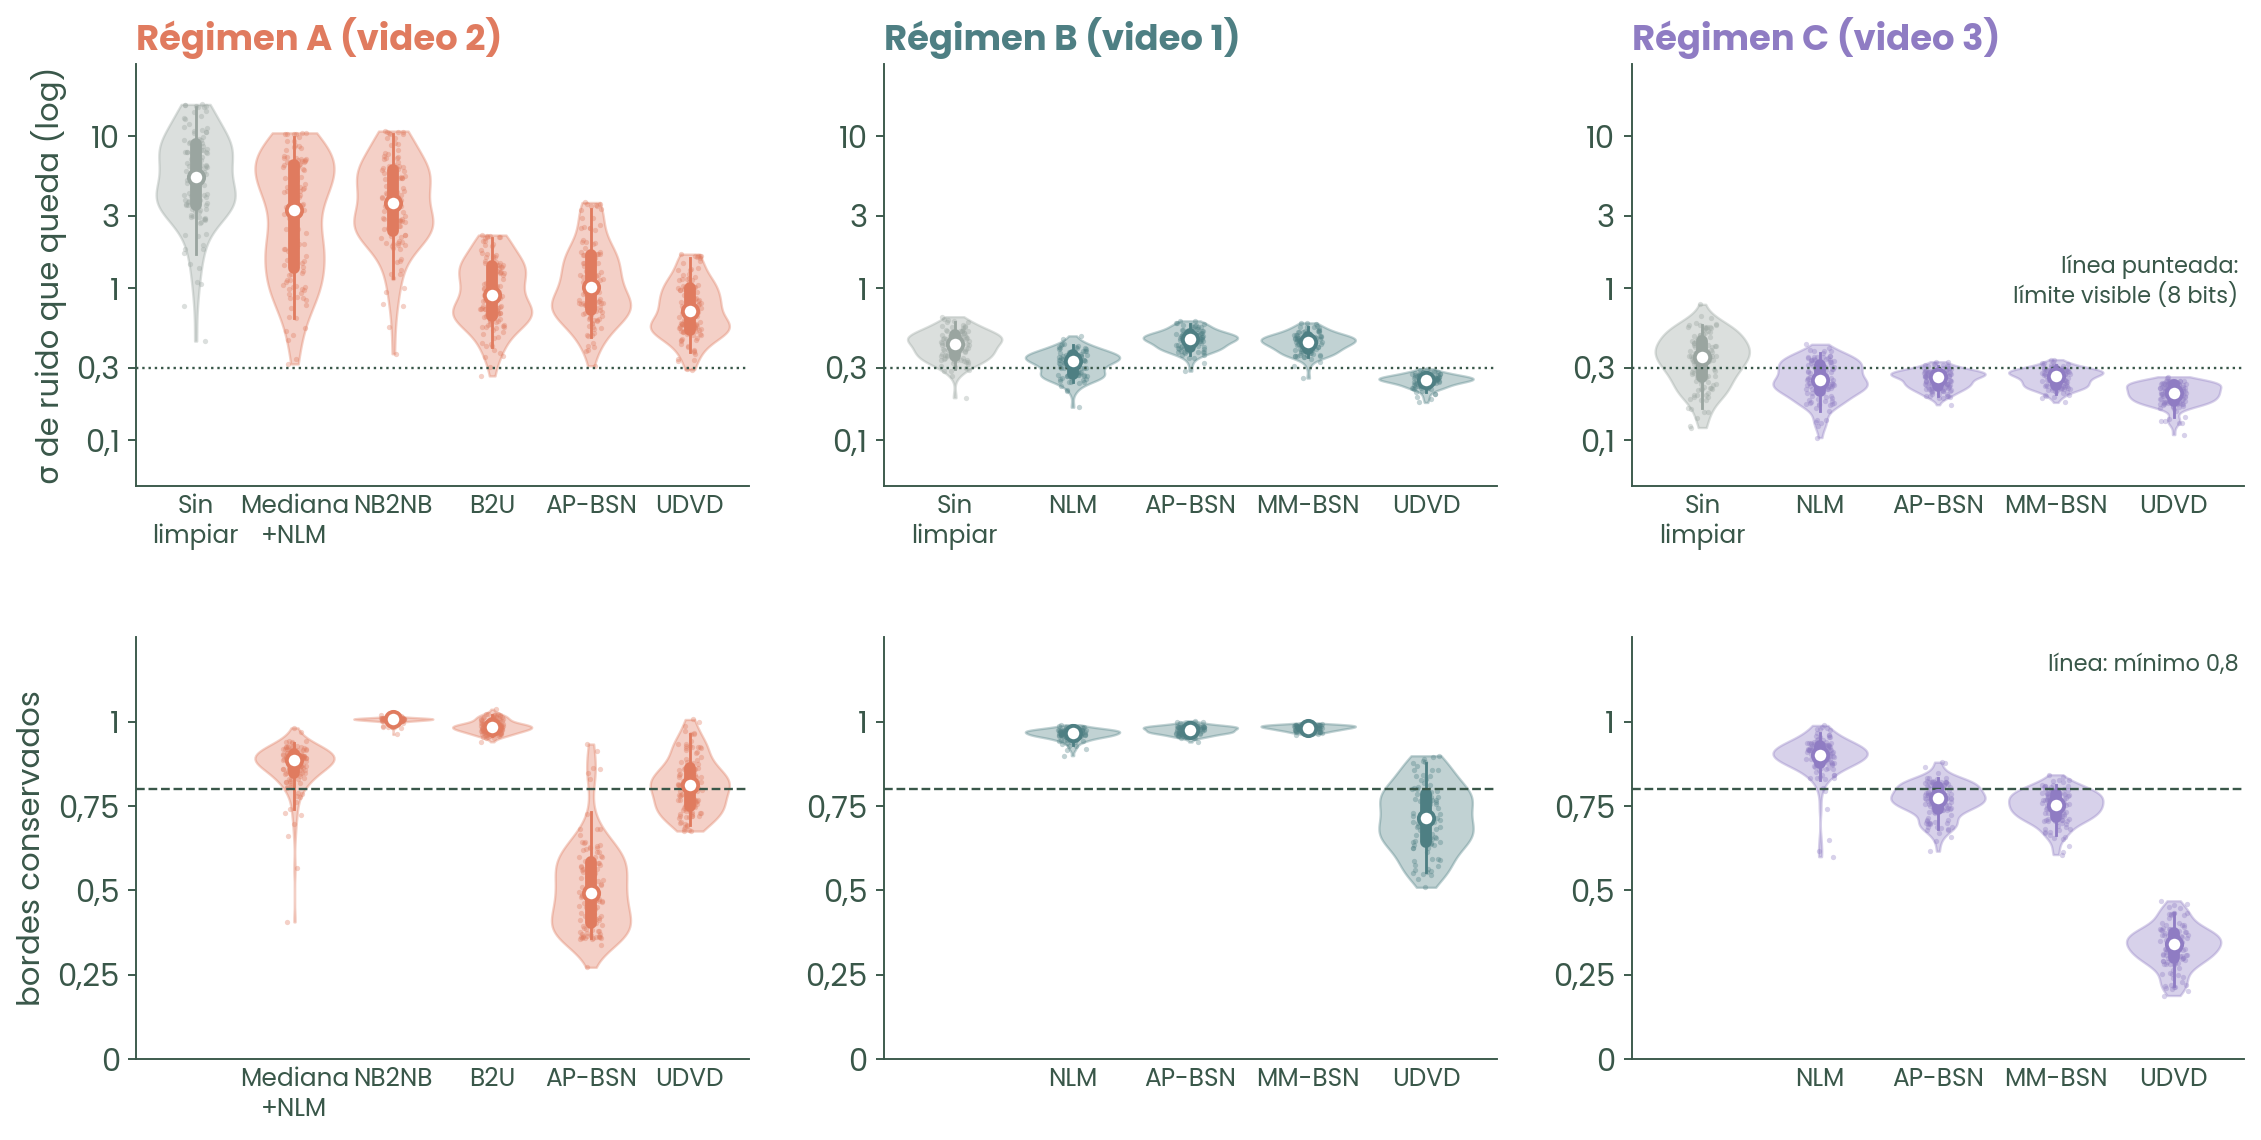
\includegraphics[width=\textwidth]{figures/limpieza/ronda1_dist.png}
\caption{Primera ronda: ruido residual (arriba) y bordes conservados (abajo) por imagen, para cada método y régimen. Círculo: mediana; barra gruesa: p25--p75; línea: p5--p95.}
\label{fig:ronda1}
\end{figure}

\paragraph{Regímenes B y C (videos 1 y 3).} El ruido de estos regímenes está cerca del nivel de cuantización, así que no es visible. Lo que sí tienen son bloques de compresión, y las redes que los atenúan también desenfocan detalle real. En las dos primeras rondas la conclusión fue dejarlos sin reducción de ruido y aplicarles solo la eliminación del HUD. \pendiente{confirmar o corregir con la ronda 3.}

\paragraph{Régimen A (video 2).} Es el único con ruido visible y concentra el 74\,\% del conjunto anotado. En la segunda ronda, AP-BSN y MM-BSN redujeron el grano de 9,4 a entre 1,7 y 2,0, pero desplazaban el color; Neighbor2Neighbor y Blind2Unblind casi no limpiaron y UDVD introdujo un patrón de cuadrícula. El desplazamiento de color se corrigió tomando el brillo de la salida de la red y el color de la entrada suavizada, con lo que la razón de croma quedó cerca de 0,97.

\pendiente{ronda 3: distribución por imagen de la reducción de NIQE y BRISQUE por método y régimen (gráficas de violín), modelo ganador de cada régimen, verificación de la meta del 8\,\% y recortes comparativos.}

\subsection{Impacto sobre la detección}
\pendiente{entrenar y evaluar el detector sobre las tres versiones del conjunto con la misma partición sin fuga; reportar instancias detectadas y recall por clase, con la verificación del $\pm 5\,\%$.}

\subsection{Descripción de segmentos con modelos de lenguaje visual}
\pendiente{dense video captioning sobre los videos limpios: modelo, prompts, segmentos localizados y evaluación cualitativa.}
